\subsection{Actuators}
    \dots\textit{introduction}\dots

    \subsubsection{Thrusters}
        % https://www.cubesatshop.com/wp-content/uploads/2017/04/ENP-IFM-Nano-Thruster-Product-Overview.pdf
        % https://blog.satsearch.co/2019-07-10-cubesat-thrusters-an-overview-of-in-space-propulsion-products-for-small-satellites
        \dots\textit(principle of operation)\dots
        
        Parameters:
        \begin{itemize}
            \item Thrust range;
            \item Nominal thrust \textit{(find a way to model change)}
            \item Specific impulse \textit{(and ranges)}
            \item Max propellant
            \item Total impulse
            \item Power consumption \textit{(at nominal thrust)}
            \item Mass
            \item Dimensions?
            \item Hot standby Power
            \item Time delay to control
            \item In both directions
        \end{itemize}
        
        \dots\textit{description of implementation}\dots

        % Bang-bang: https://apps.dtic.mil/dtic/tr/fulltext/u2/a291803.pdf
        % /resources/noise_description.pdf

        \begin{figure}[H]
            \centering
            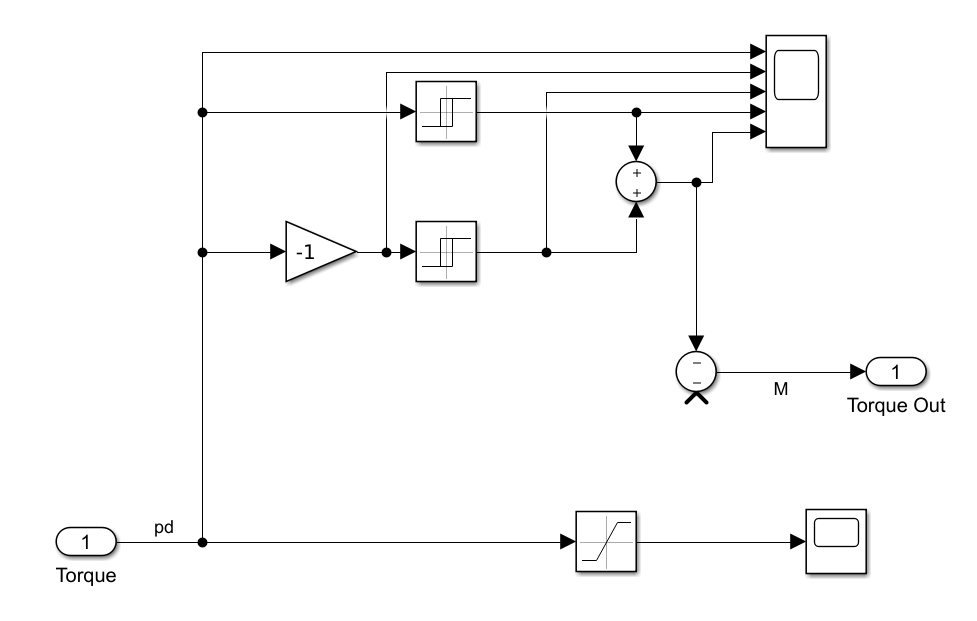
\includegraphics[width=1\textwidth]{2-toolbox/thru_simulink.png}
            \caption{Simulink Thrusters model}
            \label{fig:thru_simulink}
        \end{figure}

    \subsubsection{Reaction Wheels}
        % Ideal to real: Bearing Noise, Transport Delay, Saturation, Quantization.
        
        Fast attitude control can be also achieved by the use of reaction wheels - mechanisms consisting of rotating flywheel and proportional electromagnetic torquer, such as DC motor. This allows for very precise attitude maneuvers, with the possibility to eliminate most disturbance torques. Reaction wheels operate around at a non-zero reference speed and change in their angular velocity imposes corresponding torque on the spacecraft. The disadvantage of this solution is that reaction wheels have fixed operating range and to achieve higher angular velocities for the spacecraft, the wheels have to be desaturated using another actuators. In CubeSats, for example, most commonly this would be solved by the addition of magnetorquers.

        In fast attitude control the motion about each spacecraft body axis can be considered to be decoupled from motion about two other axes. The equations of motion that describe the influence of reaction wheels angular velocity $\dot{q_w}$ on total angular momentum $H$ are as follows:
        
        % \begin{equation}
        \begin{align}
            I_y\dot{q} &= Ni+Q_f+Qdy\\
            \dot{\Theta} &= q\\
            J\dot{q_w} &= -Ni-Q_f\\
            Ri &= e - N(q-q_w)\\
            Q_f &= -c(q-q_w)\\
            H &= I_yq + Jq_w
        \end{align}
        % \end{equation}

        Where $e$, $i$, $R$ are respectively steering voltage, current in DC motor and armature resistance. $N$ is torque per unit current and $c$ is viscous friction coefficient. Said equations were modelled in the toolbox with a following diagram: 
        
        \begin{figure}[H]
            \centering
            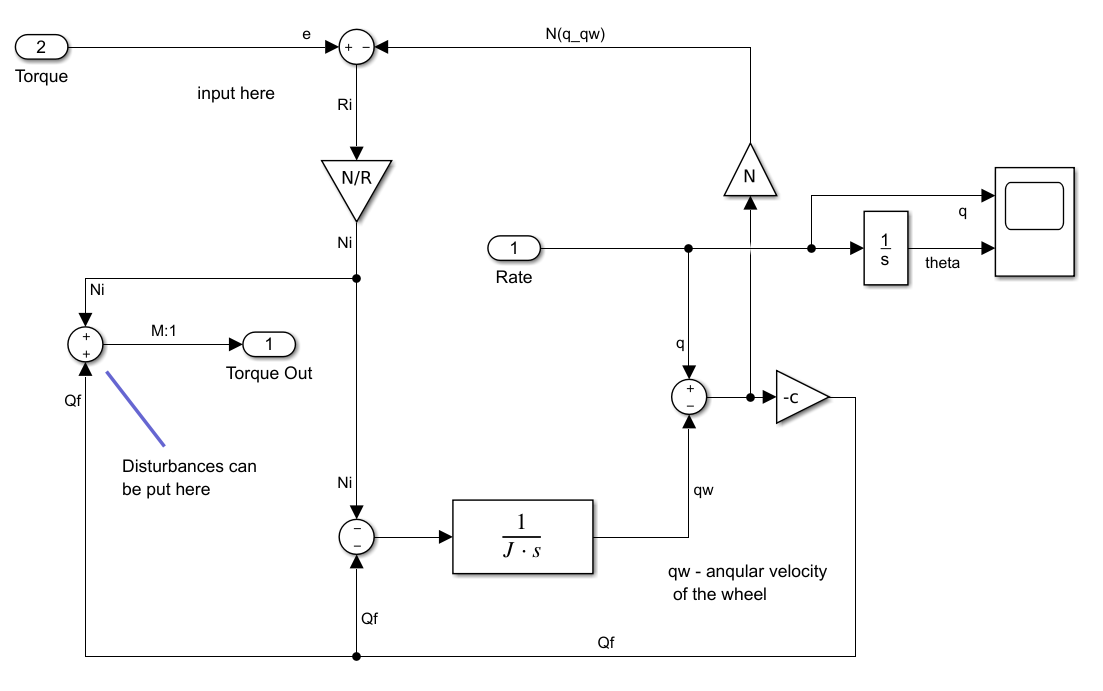
\includegraphics[width=1\textwidth]{2-toolbox/rw_simulink.png}
            \caption{Simulink Reaction Wheels model}
            \label{fig:rw_simulink}
        \end{figure}

        The problem with modeling off-the-shelf reaction wheels is that datasheets rarely provide the value of viscous friction coefficient $c$ in the DC motor, therefore in \ac{scars} it is considered to be an optional parameter. 
        
        % Therefore to model this kind of actuator, \ac{scars} requires the user to only input following data, with $c$ being optional:
        
        % sources: bryson and this funny magnetorquer stuuff
        
        % \subsubsection{Gimbaled Momentum Wheel}

        %here goes the table


    \subsubsection{Magnetorquers}
        % sources - "magnetorquer and nice stuff" pdf and sidi maybe?
        A magnetorquer is an attitude actuator which uses Earth's geomagnetic field to generate controlling torque. The active part in the magnetorquer is the solenoid, which generates the magnetic dipole moment proportional to the current conducted by the coil. This interaction is described with the following equataion:

        \begin{align}
            \tau_B = M \times B
        \end{align}

        Where $\tau_B$ is mechanical torque acting on the spacecraft, $M$ the generated magnetic moment inside of it and $B$ is the magnetic field density. In matrix form it is:
        \begin{equation}
            \begin{bmatrix}
            \tau_{Bx}\\ 
            \tau_{By}\\ 
            \tau_{Bz}
            \end{bmatrix}
            =
            \begin{bmatrix}
            0 & B_z & -B_y\\ 
            -B_z & 0 & B_x\\ 
            B_y & -B_x & 0
            \end{bmatrix}
            \begin{bmatrix}
            M_x\\
            M_y\\
            M_z
            \end{bmatrix}                
        \end{equation}

        % interesting problem with B matrix being singular, SIDI page 186 (204 in pdf)

        The drawback of using magnetorquers for attitude control is that they are unfit for fast maneuvers. Moreover, since Earth's magnetic field density is inversely proportional to cube of distance from Earth's center, then without high grade sensors or on-board models, they don't allow for precise maneuvering on higher orbits.

        \begin{figure}[H]
            \centering
            \includegraphics[width=1\textwidth]{example-image-a}
            \caption{Magnetorquers model}
            \label{fig:mag_simulink}
        \end{figure}


    \subsubsection{Drag Sail}
        Drag sails use the occurrence of partial atmosphere (described in \ref{toolbox:atmosphere}) to lower satellite's tangential velocity and therefore to quicken the deorbitation of the spacecraft. The premise is to increase area-to-mass-ratio by deploying a large and lightweight structure near the planned end-of-life of the spacecraft. Due to this operating principle, drag sails are only relevant for low and medium mass spacecrafts and are applicable only on \ac{leo}. To calculate the perturbing acceleration following equation is used:
        \begin{equation}
            F = -\frac{1}{2}\rho C_d A v^2sin\alpha
        \end{equation}
        Where $alpha$ is the angle between the sail's plane and satellite's velocity vector. For now the moment of sail's deployment is not simulated in \ac{scars} toolbox.

